\documentclass[iop]{emulateapj}
\usepackage{graphicx,pdfpages,array,amsmath}
\usepackage{xr,natbib}

\externaldocument{sections/setup_and_terminology}
\externaldocument{sections/transiting_planet_model}
\externaldocument{sections/limb_darkening}
\externaldocument{sections/visibility}
\externaldocument{sections/model_flux}
\externaldocument{sections/model_validation}
\externaldocument{sections/model_lightcurves}
\externaldocument{sections/complexity}
\externaldocument{sections/results}
\externaldocument{bibliography_astro}

\newcommand{\fmod}{\mbox{$f_{mod,i}$}}
\newcommand{\chisq}{\mbox{$\chi^2$}}
\newcommand{\fobs}{\mbox{$f_{obs,i}$}}
\newcommand{\vij}{\mbox{$V_{ij}$}}
\newcommand{\bj}{\mbox{$B_{j}$}}
\newcommand{\sigi}{\mbox{$\sigma_{i}$}}

\begin{document}
\title{Eclipse Mapping Code}
\author{Woody Austin}

\nocite{*}

\begin{abstract}
pass
\end{abstract}
\maketitle

\bibliographystyle{plainnat}
\setcitestyle{author year,round,semicolon,aysep={}}

\linespread{0.9}
\selectfont

\setcounter{tocdepth}{2}
\addtocounter{page}{0}

\clearpage

% INTRO
%The program is designed to model exhibit variability 
%in their light curve due to starspots rotating in and out of view on the surface of the star as
%well as features

%Section 1 Model, then subsections until validating the model
%Put in all of the figures


\externaldocument{tech_eclipse_text}

\section{Set-up and Terminology \label{terminology}}
The eclipse mapping program described in this paper derives a model for the relative surface brightness of a transiting planet host star when given a single band, short cadence light curve of the target as an input. Each run of the program produces a static map of the stellar surface. By applying the code to a series of short segments of the light curve, we are able to extract information about the time evolution of the star's surface brightness.  

In order for the program to create a brightness map, the physical properties of the star and the planet must be provided. Stellar rotation period, temperature of the star, orbital period, orbital separation, impact parameter, and transit duration are all required in order to produce an adequate model of the physical system. The star is assumed to be rotating as a uniform solid body. In addition, we require the spin-axis of the star  to be aligned with the orbital axis of the planet and the planet to be on an approximately circular orbit. These criteria are both met for our test object, Kepler-17 \cite{}.

Other inputs to the code determine how the model is able to fit the data. Choices include the binning cadence for both in and out-of-transit points of the light curve, the number of boxes and stripes there should be in the surface map, number of days per individual brightness solution or {\it window}, the number of days to increment each window, and which type of data to use (PDCSAP or SAP).

In order to efficiently describe the details of our program, the geometry of the problem must be defined and some basic terminology must be established. We divide the stellar surface into a series of large {\it regions}, as shown in Figure~\ref{fig:CoRoT}. While describing our program in this paper, the regions along the line of transit will be called {\it boxes}; the total longitudinal regions will be called {\it longitudes}; and the longitudinal regions with the box areas subtracted will be referred to as {\it stripes}. When talked about as an ensemble or when the distinction is unimportant, these regions will be referred to as just that - {\it regions}.

%Typically, %causing the regions to rotate in and out of view over time.  
%The surface brightness, $b_j$, of
%each region is held constant 

%longitudinal stripes. Additionally, we add a set of boxes that lie along the path of the eclipsing planet

\begin{figure}[h]
	\centering
	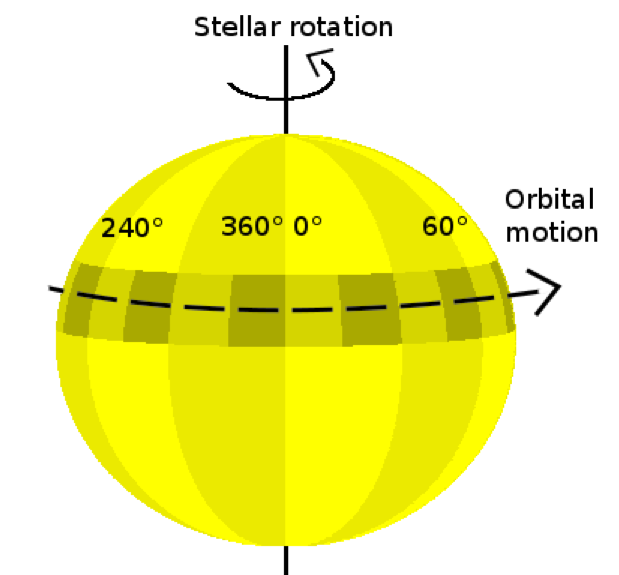
\includegraphics[width=.5\textwidth]{images/modelGeometry.png}
	\caption{CoRoT brightness map.}
	\label{CoRoT}
\end{figure}


Our program calculates the model flux at each time step, by summing over the surface of the visible sphere according to:

\begin{equation}
	\fmod = \sum_j V_{i,j}b_j, 
\end{equation}

where $b_j$ is the brightness per unit area for region $j$ and $V_{i,j}$ is the {\it visibility} of that region at time, $i$.


This model flux has two parts: a visibility and a brightness value. The amoeba determines the brightness values while the visibility values are pre-defined as described in section~\ref{vis}. Both of these apply to a set of $j$ regions. The planet will occlude only the boxes and will do so only during a transit. The longitudes' brightness values are defined as:

\begin{equation}
Z_j = \frac{S_j - \frac{c}{q} \sum_{j=1}^{q}B_j}{1- c}
\label{z_val}
\end{equation}

Where $q$ is the ratio of $n_{boxes}$ to $n_{stripes}$ and $c$ is the ratio of the total eclipsed area to the non-eclipsed area. $c$ can be calculated by the same set of integrals that will be used for the visibilities. If the Amoeba algorithm is given the set of boxes and stripes, they will be able to vary to offset each other creating a "zebra" pattern in the brightness map.  The longitude values from equation~\ref{z_val} create parameter independence by warping the chi-squared space so that such a case is less likely to become a local minimum. The Amoeba algorithm takes the set of box brightness guesses and longitude brightness guesses as inputs. During each call of the chi-squared algorithm the stripe values are calculated from the longitudes and boxes. The boxes and the stripes are then used to calculate the model flux.


\vspace{9mm}
\externaldocument{tech_eclipse_text}

\subsection{Visibility Calculations of Regions \label{vis}}
The visibility of each {\it region} is defined in Equation~\ref{vis_equation} to be the projected area along the line-of-sight modified by the limb-darkened intensity. This quantity varies as the star rotates. For example, flux from a {\it region} in the middle of the backside of the star will contribute nothing to the overall luminosity at that time. Half a rotation period later, that same {\it region} will be in the center of the front of the star and contribute a maximal amount of flux.

\begin{equation}
	V_{i,j} = \int_{\phi_1}^{\phi_2} \int_{\theta_1}^{\theta_2} \frac{I(\theta, \phi)}{I(0)} \sin^2{\theta}\cos{\phi}\,\mathrm{d}\theta \, \mathrm{d}\phi
	\label{vis_equation}
\end{equation}

The visibility equation is simply the integral of the dot product of the spherical surface element, d$A$ and the unit vector, $\hat{x}$, along the line-of-sight to the observer multiplied by the quadratic limb-darkening function provided in \citet{Claret2004}. $\phi_1$, $\phi_2$, $\theta_1$, and $\theta_2$ are in standard spherical coordinates and denote the angular limits of an individual {\it region}. For any type of {\it region} ({\it box}, {\it stripe}, or {\it longitude}), the limits change, but the equation remains the same. We solve this integral analytically and then substitute in the appropriate limits of integration.

To calculate the {\it longitude} visibilities, $\phi_1$ and $\phi_2$ are determined by the number of stripes, $n_s$, defined at the start of the program and then modified at each timestep based on the rotational phase of the star. The latitude limits, $\theta_1$ and $\theta_2$ are always 0 and $\pi$. For the {\it box} visibilities, the $\phi_1$ and $\phi_2$ limits are determined in the same way using the number of {\it boxes}, $n_b$. The latitude limits depend on the impact parameter and the radius of the planet such that $\theta_{1,2} = cos^{-1}(b \pm R_p)$. The {\it stripe} visibilities are calculated by subtracting the sum of the {\it box} visibilities in a given longitude range from the {\it longitude} visibility in the same range. Simplifying the calculation of the {\it stripe} visibilities is the primary reason for choosing the number of {\it boxes} to be an integer multiple of the number of {\it stripes}. The sum of all {\it stripe} and {\it box} visibilities at any timestep should be equal to 1.0 by definition except during a transit. 

When the planet passes in front of the star, the apparent brightness of the system diminishes by an amount related to the area of the planet. To incorporate this effect in the model flux, we modify the visibilities of the {\it boxes} that are blocked by the planet during a transit. At each timestep, we use the orbital properties of the planet and the rotational phase of the star to determine which {\it boxes} are blocked, either fully or partially, by the planet. Then we calculate the intersection of the planet with each of those {\it boxes} on the projected surface of the star. The resulting value is multiplied by the average limb-darkened intensity in the {\it box} and subtracted from its unocculted visibility. We approximate the occulted {\it box} by a cartesian rectangle intersecting a circle and use standard Euclidean geometry to determine the area of the sector that is contained within the {\it box}. To verify that the simplifying approximation that each of the {\it boxes} is a cartesian rectangle on the surface of the star is reasonable, we show a plot of our transit model over the \citet{MandelAgol2002} model generated from the same physical planet properties. The difference between the two models is less than $<*********************\%$. A typical {\it box} visibility curve is shown in Figure~\ref{box_vis}. In addition, we provide additional details about the visibility caluclations in Appendix~\ref{vis_appendix}. 

%Near the limbs, the curvature of the boxes as compared to the cartesian rectangles becomes more extreme, but the boxes are smaller and thus the absolute error is smaller. 

\begin{figure}[h]
	\centering
	\includegraphics[width=.5\textwidth]{images/transit_check.eps}
	\caption{Our model transit is shown on top while the Mandel \& Agol model is shown on the bottom. The difference between the two models is less than x\%.}
	\label{transit}
\end{figure}
*********Make this eps
\begin{figure}[h]
	\centering
	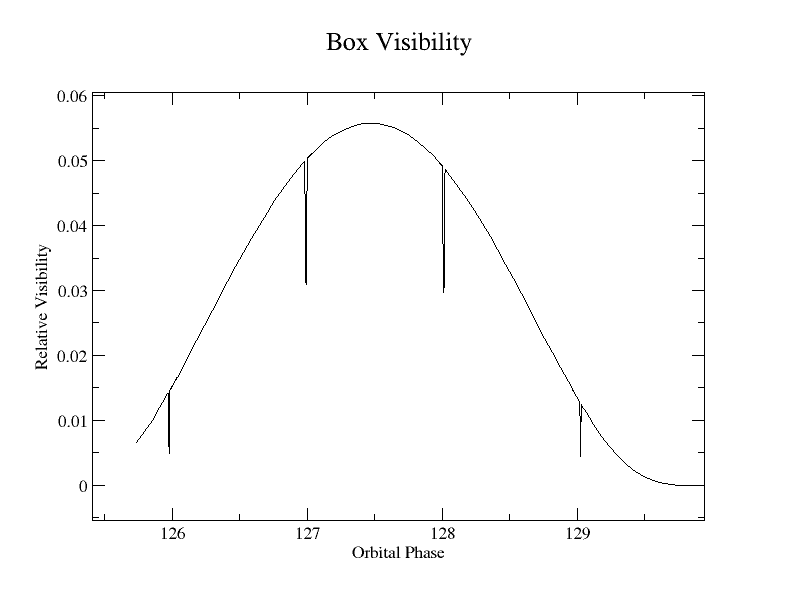
\includegraphics[width=.5\textwidth]{images/box_vis.eps}
	\caption{An example visibility curve for one {\it box}. This is "box 0", or the box whose left edge is on the left limb of the star at time 0 (the given epoch). This was generated for a system with the same parameters as Kepler-17, later shown in Section~\ref{validation}. $\theta_1$ and $\theta_2$ are $81.52^\circ$ and $96.4^\circ$ respectively.}
	\label{box_vis}
\end{figure}
\vspace{9mm}
%\subsection{The transiting planet model \label{transit_model}}
To model the starspot features within the transit portions of the light curve, we must explicitly model how the transits of the planet affect the amount of flux that reaches the observer. The visibility of the transits is comprised by the portion of the star that the planet occludes during transit and limb darkening effects. As discussed in Section~\ref{vis}, the planet will only transit along the boxes contained within the latitudes at $cos^{-1}(R_p \pm b)$. 
 
The first step in determining the visibility occluded by a planet at a given time step involves geometry which will be extended to ten cases contained in Table~\ref{cases}. The simplifying approximation that each of the boxes is a cartesian rectangle when it is projected onto the surface of the star is made. The midpoints of the edges of the cartesian rectangle are the same as the midpoints of the projected box edges. The top and bottom latitude limits of the cartesian rectangles are the same as those of the projected rectangles. Although this is not entirely accurate, it is a good approximation.  When a cartesian rectangle overestimates a portion of the projected box, it must also underestimate a similar but not necessarily equal portion of the box. Near the limbs, the curvature of the projected boxes as compared to the cartesian rectangles becomes more extreme, however the cartesian rectangles become smaller. In these cases the relative area misappropriated may be larger, the absolute error is smaller.

The calculations for the eclipsed visibility geometry are shown in full in ~\ref{trans_appendix}.


\vspace{9mm}
\externaldocument{tech_eclipse_text}

\subsection{Limb Darkening}
To actually calculate the limb-darkening, a quadratic limb-darkening law is used.
\begin{equation}
   \frac{I(\psi)}{I(0)} = 1 - c_1 (1 - \mu) - c_2 (1 - \mu)^2
\end{equation}
Here, $\mu$ is the cosine of the angle between the line of sight and the normal at the point at which you are trying to calculate the limb darkening. Because stars are so distant, this can be approximated as $\hat{x} = R^* \sin{\theta}\cos{\phi}$, but $R^{*}$ is defined as 1.0 throughout all calculations.

To complete the limb darkening model, the average value in one of the regions is calculated at every timestep. This is done analytically from the integral:

\begin{equation}
\begin{split}
    \frac{1}{V_{i,j}} \int_{\phi_1}^{\phi_2} & \int_{\theta_1}^{\theta_2}  (1 - c_1 (1 - \sin{\theta}\cos{\phi}) \\ &- c_2 (1 - \sin{\theta}\cos{\phi})^2) \sin{\theta}\cos{\phi}\,\mathrm{d}\theta \, \mathrm{d}\phi
\end{split}
\end{equation}

This works well for limb-darkening determination in each region, but care must be taken when calculating limb darkening for the eclipse. Rather than calculating equations of limb darkening for the eclipse directly as in Mandol \& Agol 2000, the ratio of the limb-darkened eclipsed region to the non-limb-darkened eclipsed region is used. If the number of regions in eclipse is not high enough, a boxy limb-darkening approximation to the transit path is produced using this scheme. This happens because the planet is moving too quickly relative to the surface of the star given the in-transit binning cadence. To fix this, the ratio of the limb-darkened to non-limb-darkened regions is calculated for multiple sub-regions. This gives a finer grain approximation to the real value.


\vspace{9mm}
\externaldocument{tech_eclipse_text}

\subsection{Solving for the brightness values \label{flux}}
The goal of the program is to identify a realistic brightness distribution of the stellar surface. We employ a standard chi-squared minimization routine, the Amoeba Algorithm, to find the optimum brightness values, $b_j$, that, when multiplied by the visibilities as described above, produces a model light curve according to that matches the observed data. This model light curve is produced according to Equation~\ref{model_flux}. The Amoeba Algorithm is a minimization tool that works well for small numbers of dimensions (regions in this case) and which will always converge to some minima (although not necessarily absolute) \citep{NR}. Given an initial set of brightness values given pre-defined visibilities as described in section~\ref{vis}. Both of these, brightness values and visibilities, apply to a set of $j = n_{boxes} + n{stripes}$ regions. The planet will occlude only the boxes and will do so only during a transit. The longitudes' brightness values are defined as:
\begin{equation}
	\chi^2 = \sum \frac{(\fmod - \fobs)^2}{\sigma_i^2}
\end{equation}



For a given set of data the brightness values cannot change using our technique. To remedy this, each month (or quarter) of data is divided into smaller intervals called {\it windows}. By moving the start and end times of the windows by small amounts, information about the evolution of starspots can be inferred. Previous estimates on the timescale of starspot evolution report that it occurs on the order of 10-30 days ***********cite someone*******. This works well with the model described here. The model does a better job of fitting smaller sections of data than larger ones. *******Note about striping*******


The Amoeba Algorithm is used to do the actual minimization. The algorithm runs quickly and will always converge given any set of inputs. The largest downside (of most optimization algorithms) is that it cannot distinguish between local and absolute minima. This becomes especially apparent when choosing an initial set of brightness guesses for the simplex structure. Because the average brightness of the star is 1.0, the initial conditions for the simplex structure are $n_{sb} + 1$ brightness sets of $n_{sb}$ values where $n_{sb} = n_{stripes} + n_{boxes}$ and every element is in the simplex is 1.0. A different (orthogonal) basis vector $e_i$ times a scale factor, $s$, is then added to each of the $n_{sb} + 1$ sets. When the scale factor is too large, the Amoeba converges on answers that are not likely real. When the scale factor is too small or non-existent, the Amoeba is more likely to vary all regions in order to converge to a solution rather than just the regions that differ from the average value.




\begin{equation}
%Z_j = \frac{S_j - \frac{c}{q} \sum_{j=1}^{q}B_j}{1- c}
S_j = Z_j (1 - c) + \frac{c}{q} \sum_{j=1}^{q}B_j
\label{z_val}
\end{equation}
%Changed the above equation... switched Z and S values.

Where $q$ is the ratio of $n_{boxes}$ to $n_{stripes}$ and $c$ is the ratio of the total eclipsed area to the non-eclipsed area. $c$ can be calculated by the same set of integrals that will be used for the visibilities. The Amoeba algorithm is given the set of box and longitude visibilites $\{b_1, ..., b_j, z_1, ..., z_n\}$. When the planet is not transiting, the only information available is about the total longitudinal brightness information. Within the chi-squared call of the Amoeba algorithm, the box and stripe visibilities and brightnesses are calculated as a way to blend the parameters together and get information about the overall longitude. This allows the use of boxes and stripes whose sum can be thought of as the longitude values in the Amoeba while still getting information about the boxes and the longitudes independently. This is called parameter interdependence. This appears to encourage the Amoeba Algorithm to navigate to a better local minima than if this process of creating parameter interdependence and using optimal variables were omitted. 

\vspace{9mm}
\externaldocument{tech_eclipse_text}

\section{Validating our model \label{validation}}
%Things that were in the version that got lost:
%	Rework first two sentences
%	3) Explain that we chose 11/22 as per the section before this


Extracting a two dimensional brightness map by fitting a model to a one dimensional light curve can result in degenerate solutions.  There is no way of knowing what the brightness values of a real system should be {\it a priori}. To remedy this, we produce synthetic light curves using our definition of model flux, a set of visibilities, and a known set of input brightness values. The average brightness on the surface of the star is defined to be 1.0. This is the default value for this known set of input brightness values. To simulate starspots, we darken regions by giving them a brightness value of less than 1.0. For example, if we want to simulate a group of spots in only one {\it box}, we would set all of the input brightness values to 1.0 except for one {\it box} that has the value 0.90. One the spots are darkened, the flux is then integrated at each time step over all of the {\it regions}. There are currently 11 synthetic light curves with different spot configurations that we test with our system, but only a subset will be detailed in the paper.

\begin{table}
\begin{center}
  \begin{tabular}{l | l}
    Parameter Name & Value \\ \hline
    Rotation Period & 11.89\\
	$\frac{R_p}{R^{*}}$ & 0.129530 \\
	Limb Darkening Coefficient 1 & 0.4282\\
	Limb Darkening Coefficient 2 & 0.2514\\
	Orbital Period & 1.485711\\
	Orbital Epoch & 352.678035\\
	Orbital Separation & 5.670\\
	Impact Parameter & 0.01800\\
	Transit Duration & 0.094775\\
  \end{tabular}
\end{center}
\label{models}
\end{table}

We want our synthetically produced light curves to mimic light curves from real systems. To ensure that this happens, we adopt the stellar, planetary, and orbital properties directly from the Kepler-17 system provided in \citet{Borucki????} ****Cite the correct parameter place and shown in Table~\ref{parameters}. These parameters are then used to create the visibilities, as described in Section~\ref{visibilities}, and determine an appropriate number of stripes and boxes for the system as described in Sections~\ref{visibilities} and ~\ref{flux}. For the Kepler-17 system and for our synthetic systems, we choose the number of {\it stripes} and {\it boxes} to be 11 and 22 respectively.

A typical spot on a real star is anywhere from 500 to 1000 degrees cooler than the rest of the stellar surface. This corresponds to about 0.67 the brightness of an average part of the star in the starspot \citep{Walkowicz2013}. The {\it regions} in our synthetic systems are designed to imitate a real star with at most 30\% spot coverage. Therefore, the brightness values in our {\it regions} vary from 1.0 down to 0.88 in the {\it boxes} (higher percentage of spot coverage) and down to 0.91 in the {\it stripes}. 

When the light curves are produced in this way, they do not have any noise. This is clearly a bad imitation of a real system. We introduce Gaussian noise with standard deviations based on the average photon error counts provided in the table at \citet{noise_levels_table}****Noise level table. We try to recover the brightness values for noiseless, 12th magnitude noise, and 14th magnitude noise synthetic light curves. We show examples of the same light curve with different levels of noise in Figure~\ref{noise_comp}. Kepler-17 itself is a fourteenth magnitude star.

\begin{figure}
	\centering
	\includegraphics[width=.5\textwidth]{images/noise_levels.eps}
	\caption{Comparison of noise of models. The noise for these models was based off of error counts similar to a given magnitude Kepler star. Our tests included models with no noise in blue, simulated 12th magnitude noise (441 counts per million) in red, and simulated 14th magnitude noise (1620 counts per million) in green \citep{noiseCounts}.}
	\label{noise_comp}
\end{figure}

The in and out-of-transit binning cadences also mimic how we would solve for a real system. Because so many points exist out of transit and the trends from larger, possibly polar spots tend to have longer timescales, a low binning cadence is desired for out-of-transit binning. For these example solves, the out-of-transit binning cadence is 95 Kepler short-cadence time steps (58.85 seconds) per bin. The in-transit binning cadence is set at a higher frequency in order to remain sensitive to small scale variations in the light curves due to small scale starspots in the path of the planet. For these example solves, the in-transit binning cadence is set to three Kepler short-cadence time steps per bin.

Our predetermined set of brightness guesses $B = \{b_1, b_2, ..., b_{nboxes}, b_{stripes}, ..., b_j\}$ remains constant over then entire period of data in question (usually a month of Kepler short-cadence data). This is not a good approximation to real data as it does not include any notion of starspot evolution. However, over the short period of each {\it window} the evolution is not a noticeable factor, and it makes more sense to produce the lightcurves in this way.



%While trying to verify the models, the only things that can vary for the reproduction is the number of boxes and stripes and the binning cadences. The number of stripes is chosen doing a sans-transit fit to the light curve with an increasing number of stripes until the chi-squared stops becoming significantly better. The number of boxes is chosen by calculating the relative area of the star that the planet occludes per time step. To resolve at a small scale, we want the planet to have three time steps in each box before moving on to the next one \citep{Huber2009}. Using these metrics, we chose the number of boxes and stripes for our system to be 11 and 22. 
\vspace{9mm}
\externaldocument{tech_eclipse_text}

\subsection{Producing the model light curves \label{modelLC}}
To produce the synthetic light curves, the model flux $\fmod = V_{i,j} b_j$ was used. The flux is integrated at each time step over all of the regions whose visibility calculations are the same as described in section~\ref{vis}. A predetermined set of brightness guesses $B = \{b_1, b_2, ..., b_{nboxes}, b_{stripes}, ..., b_j\}$ is used to produce a new light curve. This set of brightness values is constant over then entire period of data in question (usually a month of Kepler short-cadence data).

To simulate spots in the synthetic light curves, certain individual regions are darkened. The average brightness of the undarkened star should be 1.0 everywhere. A typical spot is anywhere from 500 to 1000 degrees cooler than the stellar surface which corresponds to about .67 the brightness of an average part of the star \citep{Walkowicz2013}. The regions in our synthetic systems are designed to approximate a star with at most 30\% spot coverage. Because of this, the brightness values in the regions vary from 1.0 down to .88 in the boxes (higher percentage of spot coverage) and down to .91 in the stripes. There are currently 11 synthetic light curves that are tested with our system, but only a subset will be detailed in the paper.

The light curves that were used to test the code had stellar and planetary parameters similar to that of Kepler 17. $P_{rot}$, $P_{orb}$, $R_p$, orbital separation, limb darkening (temperature), and transit width are all identical to the Kepler 17 system. When the light curves are produced, there is no noise. To remedy this, a simple python script generates Gaussian noise based on a Kepler-Magnitude input. 

\begin{figure}
	\centering
	\includegraphics[width=.5\textwidth]{images/noise.png}
	\caption{Comparison of noise of models. Blue is noiseless, Red is 12th magnitude, and Green is 14th magnitude Gaussian Noise.}
	\label{noise_comp}
\end{figure}

The noise for these models was based off of error counts similar to a given magnitude Kepler star. Our tests included models with no noise, simulated 12th magnitude noise (441 counts per million), and simulated 14th magnitude noise (1620 counts per million) \citep{noiseCounts}. Figure~\ref{noise_comp} shows a {\it window} of our model light curve with the three levels of noise for comparison.



%New Order:
%1) Our simulated star has X Stripes and Y Boxes.
%2) Describe the darkening process. And give the values between .88 and 1.0. Justify the numbers that we used in the simulations. Corresponds to spot temperatures that correspond to 500 to 1000 degrees cooler than the surface of the star ****Verify that temperature number. Mention that non-modified b-values are set to 1.0
%	Insert: Table of different simulations
%		Requires coming up with a numbering scheme to generate said table
%3) Properties of star are similar to Kepler 17: list it. Go in a table.
%4) Reword the actual production to use these brightnesses described above and the visibilities instead of how it actually works in the code.
%5) Total duration of one month - similar to one month of short cadence Kepler data at the same time steps of Kepler 17
%6) No evolution in the b values over this time
%7) Add noise to the light curve. Give the sigma values corresponding to 12th and 14th.
\vspace{9mm}
\externaldocument{tech_eclipse_text}

\subsection{Testing Complexity \label{complexity}}
The ability of the program to solve for brightness values has only been tested in two parameter spaces, complexity of the spots and noise of the light curve. The noise of the curve is generated by a python script based on Kepler Magnitude noises. Models were tested for a noiseless, a 12th magnitude star, and a 14th magnitude star. There is no noticeable difference between these.
%Don't list, show a table. Model ID number, short name, modified boxes column, modified stripes column.

The complexity of the spots is determined by the number of regions that vary from the default brightness value of 1.0. The model has been tested on 11 different spot configurations. These are one box, one box and one stripe, two boxes, two boxes and one stripe, two boxes and two stripes, three boxes and one stripe, three boxes and two stripes, three boxes and three stripes, four boxes and three stripes, all boxes randomly and two stripes, and all regions randomly darkened.
\vspace{9mm}
\externaldocument{tech_eclipse_text}

\subsection{Results \label{results}}
The program does a good job of recovering the input brightness values and matching the light curves. The level of noise has some effect on the reproduction of the brightness values, but clear trends can still be seen even with simulated 14th magnitude noise. One important thing to note is that the program does not recover the correct brightness values every time, but does a good job when averaged over many windows. This means that the results are better interpreted as long term trends than as exactly correct in every window. For the synthetic light curves, starspot evolution was not introduced. However, in real systems starspot evolution would exist. This means that our program can give information about overall trends in starspot evolution, but it cannot be trusted to give the exact brightness values of a region for any given time step. 

Further, the algorithm needs at least one full period per window in order to accurately reproduce the box values. With higher noise levels, more of the lightcure must be included at once. There is a tradeoff in lightcurve fit versus avoiding systematics that stem from not having enough information to recover the brightness values. It is counterintuitive to think that the brightness values are recovered more accurately overall the worse the lightcurve fit gets, but this is true. One important thing to note is that the lightcurve fit still fits extremely well overall, but there is more variation from window to window.

In all cases, the light curve fits look good for synthetic curves and real data alike. The fit of the light curve is good irrespective of noise level in the synthetic curve. The RMS of the recovered brightness values is dependent upon the noise levels, but they are still reliably recovered even with simulated 14th magnitude noise.

We have created seven diagnostic plots to compare our synthetic light curve inputs to the model outputs recovered by the code for those same inputs. The first of these plots is the input brightness map shown in Figure~\ref{model_map}. This shows every region on the star and the relative brightness values of each region that was used to create the corresponding synthetic light curve that is then fed into the eclipse mapping code.

\begin{figure}[h]
	\centering
	\includegraphics[width=.5\textwidth]{images/model_map.eps}
	\caption{The set of brightness values used to produce a specific synthetic lightcurve. In this case, this was used to produce the 1b/ set of lightcurves (no noise, 12th magnitude noise, 14th magnitude noise).}
	\label{model_map}
\end{figure}

To visualize the brightness values, we use Figures~\ref{stripe_plot} and~\ref{box_plot}. Along the x-axis is window number defined in Section~\ref{setup}. The y-axis shows the longitude of the star. The top of the plot starts at longitude 0, and the bottom of the plot ends at longitude 360 and then wraps around.These longitudes correspond to the region numbers. This is why we must separate the box and stripe visualizations. The stripes and boxes occupy the same longitude space. Each "pixel's" color is indicative of the brightness value for a given region during a given window. Each vertical strip shows a complete set of box or stripe brightness values for one window. Each horizontal strip shows the recovery for the same region over every window. The value on the far right, beyond the black separator, is the input brightness value for the synthetic light curves. You can compare the recovered brightness in that pixel with all of those in the same region to the left on the same horizontal slice.

\begin{figure}[h]
	\centering
	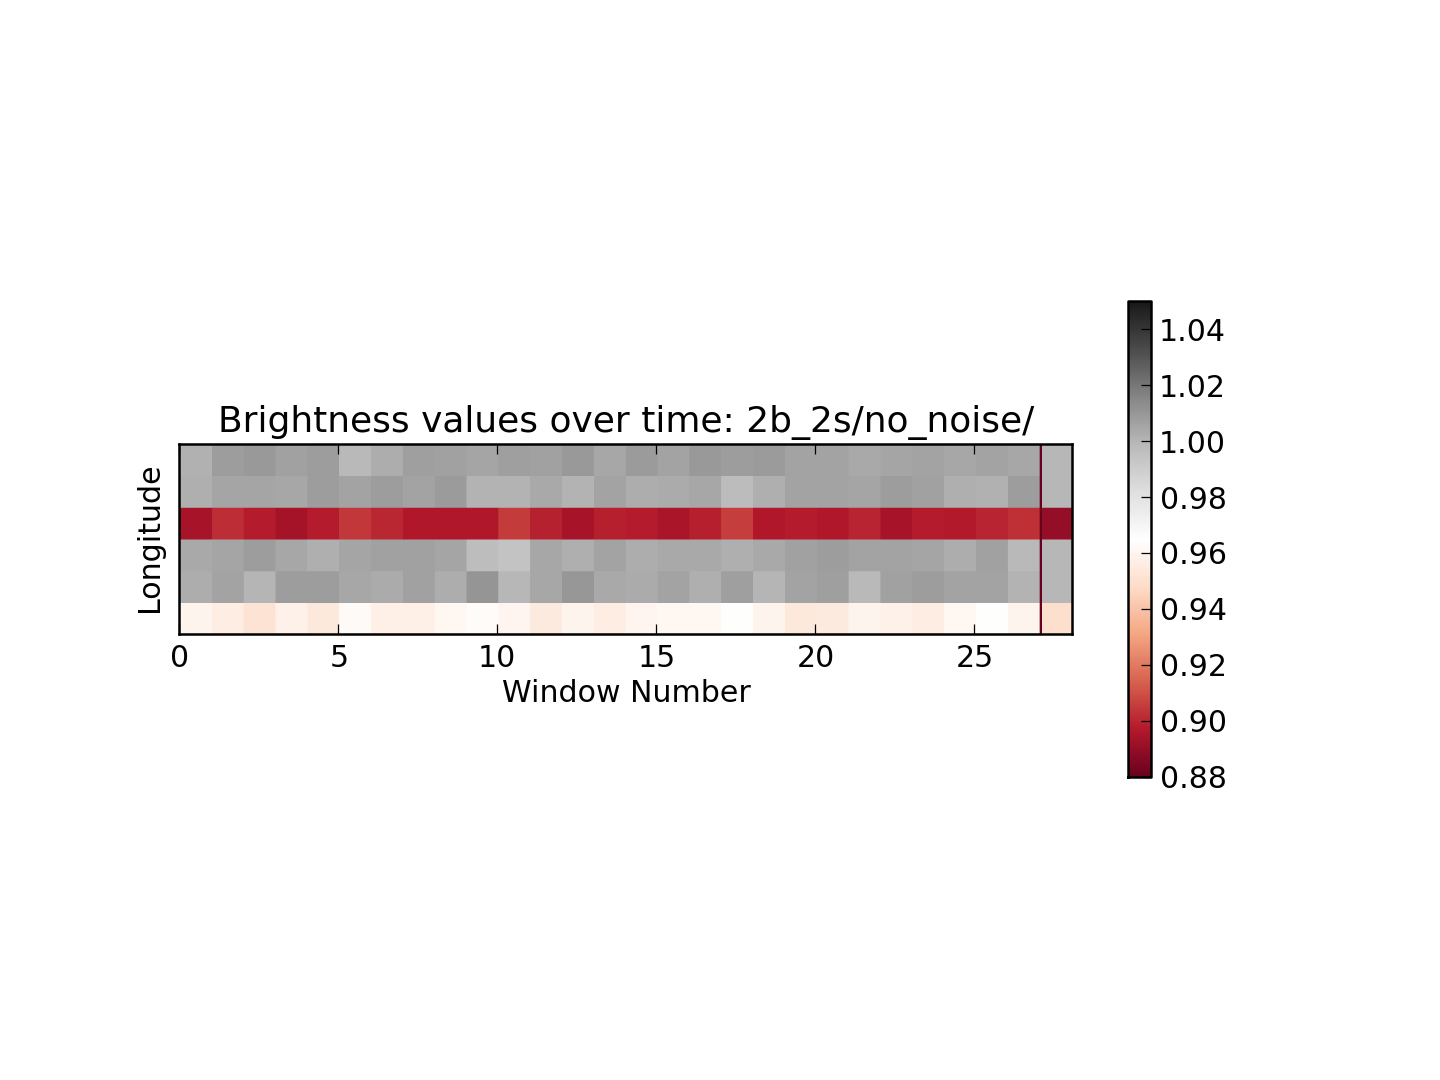
\includegraphics[width=.5\textwidth]{images/stripe_plot.eps}
	\caption{Recovered stripe brightness plot versus window number. This plot is for the no noise model with 1 box darkened. Note the desired values on the far right.}
	\label{stripe_plot}
\end{figure}

\begin{figure}[h]
	\centering
	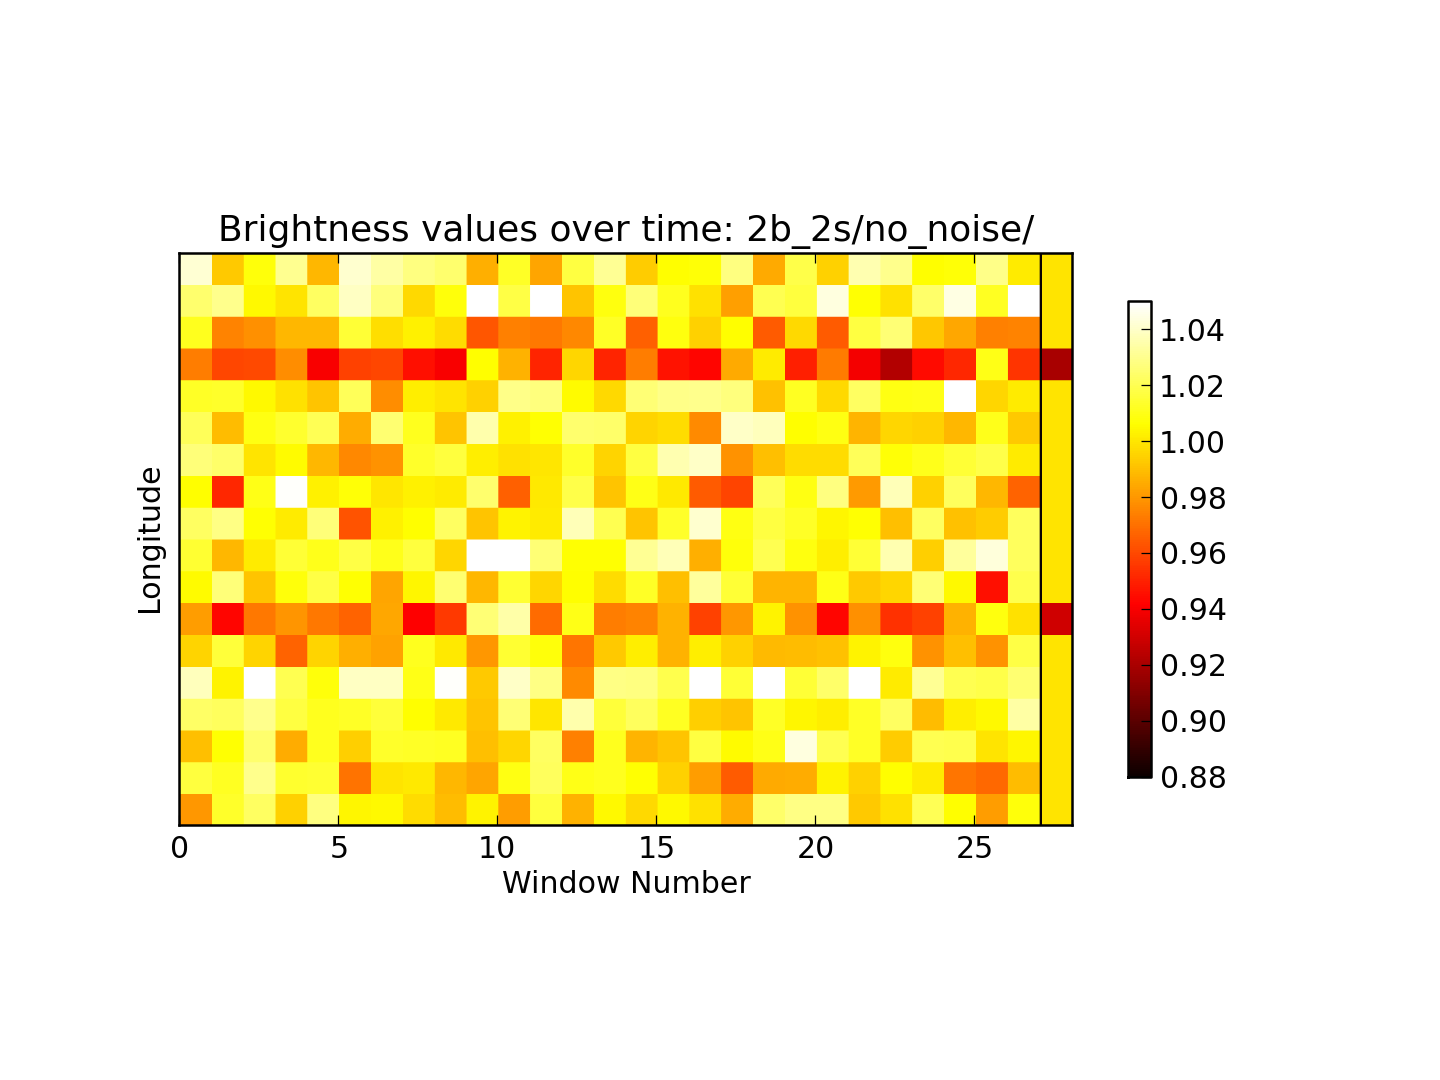
\includegraphics[width=.5\textwidth]{images/box_plot.eps}
	\caption{Recovered box brightness plot versus window number.  This plot is for the no noise model with 1 box darkened. Note the desired values on the far right.}
	\label{box_plot}
\end{figure}

An important thing to note, that should be evident from the discussion of the box and stripe brightness visualizations is that we are working with multiple windows in all cases. This makes it hard to show the brightness recovered for each individual window on the surface of a star in a compact and meaningful way. Because of this, we only show the average brightness recovered over all windows and plot it on the star similar to the input brightness map. You can see this in Figure~\ref{average_map}. For our synthetic lightcurves, this map should match the input map because there is no starspot evolution included. In a real system, a model brightness map is inadequate because evolution could occur. The average over the given time period will be correct, but it will not be reporting all of the information that has been recovered. In this situation, it would be best to produce a separate brightness map for every window or just revert to the box and stripe brightness visualizations shown in Figures~\ref{stripe_plot} and ~\ref{box_plot}.

\begin{figure}[h]
	\centering
	\includegraphics[width=.5\textwidth]{images/average_map.eps}
	\caption{Average brightness value in each region over all windows of an eclipse-mapping code run that was attempting to recover the 1b/no\_noise lightcurve.}
	\label{average_map}
\end{figure}

The next figure is the RMS of the average brightness recovered for a given region over all windows versus the input brightness used to produce the synthetic lightcurve shown in Figure~\ref{rms}. The red diamonds are the regions that have been modified from the default brightness of 1.0. This is only useful to verify that we recover the values used to create our synthetic lightcurves. It has no use for real data because we don't know the brightness values before running the code.

\begin{figure}[h]
	\centering
	\includegraphics[width=.5\textwidth]{images/rms.eps}
	\caption{Comparison of the average value over all windows for each region versus the input value for each region. This particular plot is for the 1b/no\_noise lightcurve.}
	\label{rms}
\end{figure}

The next plot is the lightcurve fit shown in Figure~\ref{lc_fit}. The red points are the input, synthetic lightcurve data. The black lines are the model fits. One thing to note here is that there are actually as many black lines as there are windows. Each black line is overlaid on top of the corresponding portion of lightcurve. As you can see in all cases, it looks like one line, and the fits are incredibly good. 

\begin{figure}[h]
	\centering
	\includegraphics[width=.5\textwidth]{images/lightcurve.eps}
	\caption{Light curve fit of the recovered models versus the synthetic lightcurve. This particular fit has 51 model fits overlaid on top of the red data and is the recovery for the 1b/no\_noise lightcurve.}
	\label{lc_fit}
\end{figure}

The final plot is that of the transit fits. Just like the overall lightcurve fit, there are multiple windows per transit that are being plotted. As the complexity grows, you can see this more and more. Each of these transit pages has the transits in order as you would read in English. We based our synthetic lightcurves off of the third month of Kepler-17 data. This particular data set has 20 transits, so all of our models have exactly 20 transits to recover.

\vspace{9mm}


\small
\bibliography{bibliography_astro}{}

\end{document}
